\documentclass[10pt,twocolumn]{article}
\usepackage[margin=0.75in]{geometry}
\usepackage{booktabs}
\usepackage{array}
\usepackage{graphicx}
\usepackage[numbers,sort&compress]{natbib}
\usepackage{style/shisso}
\shissorepo{github.com/ravediamond/paper-jepa-world-model}
\renewcommand{\dbltopfraction}{0.95}\renewcommand{\topfraction}{0.9}\renewcommand{\textfraction}{0.05}\setcounter{dbltopnumber}{2}
\begin{document}
\title{A small JEPA world model: the encoder knows, the predictor does not add}
\author{Ravindu Somawansa\thanks{Code, data pointers and every number's source: \url{https://github.com/ravediamond/paper-jepa-world-model}.}\\Shisso Robotics, Paris\\\texttt{ravindu.somawansa@gmail.com}}
\date{}
\maketitle
\begin{abstract}
We trained a small JEPA world model in the LeWorldModel recipe on teleoperated demonstrations of one tabletop task on a low-cost SO-101 arm, and re-tested on it every use of such a model that we found in recent world-model papers, each under a bar fixed in a public register. In exploratory probes on policy rollouts the model never saw in training, a linear readout of the encoder's final-frame latent separates success from failure as well as a hand-built colour judge (AUROC 0.95 vs 0.94) and better than a frozen DINOv2 encoder, the commanded joints or the policy's identity. The predictor does not add to it: at the grasp, the imagined latent reads the outcome worse than the current one (0.70 vs 0.82), and every use that needs a multi-step rollout, from chunk ranking to surprise monitoring and risk prediction, misses its bar. One rig, one model, one data scale.
\end{abstract}
\section{Introduction}
A world model in the sense of LeWorldModel (LeWM)~\citep{maes2026lewm} has two parts: an encoder that maps camera frames to a latent vector, and a predictor that, given the current latent and a sequence of actions, imagines the latents that follow. Both are trained together from pixels with a joint-embedding predictive (JEPA) loss. Papers built on such models propose \emph{uses} of them: ranking a policy's candidate action chunks by their imagined outcome, flagging a failure when the observed latent departs from the predicted one, reading the outcome of a grasp before it happens, planning over several time scales. Each paper reports the use that worked, on its own robot and data.
We take the opposite view of one model. We trained a single small JEPA world model on one arm and one task, and re-tested on it every use we could take from the literature. Each re-test is a row of a register: a bar written down before the result where we could, a dataset, a result and a verdict. Pre-registration here means only that: the bar and the decision rule are committed to the repository before the number exists. Audited against the commit history, all 20 rows match a pre-registration record; 19 bars were committed before their result and 1 in the same commit as its result (the two-level hierarchical progress use). One row, the on-device latency of the pretrained RoboJEPA and V-JEPA 2.1 encoders~\citep{zholus2026robojepa,murlabadia2026vjepa21}, is not a use of our model. Of the 20 rows, 3 pass, 1 is met as predicted, 2 are not proven, and the remaining 14 fail or are no-go.
On the 69 rollouts, and in exploratory probes only, the result splits along the model. The \emph{encoder} reads the episode's outcome from the current frame, better than a frozen foundation encoder or the robot's own joint commands, and it does so at the grasp anchor too, 15 frames before the gripper first closes. The \emph{predictor}, which every forecasting use relies on, does not improve on that reading by imagining forward. The contribution is threefold: the register itself, with an audit of how every use loaded the checkpoint (Table~\ref{tab:register}); exploratory controls that separate encoder from predictor (Table~\ref{tab:controls}, Fig.~\ref{fig:controls}); and the exploratory reading that, at this data scale, the predictor is the weak link.
\textbf{Caveats stated up front.} The encoder readouts are linear probes fit with leave-one-session-out (LOSO) cross-validation on 69 rollouts (44 success / 25 failure, 13 sessions) with operator labels. The model was trained on teleoperation only and never saw these rollouts, but the controls were chosen after the data and are \textbf{exploratory}. Among the 3 passes, 3 have bars committed before the result, and the bar of the outcome-readout use was written retrospectively. Ordered by commit alone, without the audit, the register reads 13 bar-first and 6 same-commit.
\section{Setup}
\textbf{Robot and data.} The robot is one SO-101 arm~\citep{so101} driven through LeRobot~\citep{cadene2024lerobot}, with two cameras (top and wrist) and one task family: put a bowl into another bowl. The world model is trained on \texttt{ravediamond/so101\_bowls\_all\_trimmed} (157 training and 25 validation episodes, split by grid layout). The evaluation rollouts are \texttt{ravediamond/so101-bowls-policy-rollouts}, a separate dataset of SmolVLA~\citep{shukor2025smolvla} rollouts recorded after the world model was trained.
\textbf{Model.} Our world model, named W1 in the repository, follows the LeWM recipe~\citep{maes2026lewm}: a multi-view ViT encoder, an action-conditioned predictor and the SIGReg regulariser. It was trained on one rented GPU for \$3.30. \textbf{Controls.} The frozen DINOv2-S control is a frozen DINOv2 small encoder~\citep{oquab2023dinov2}, mean-pooled over the top and wrist views, the design of DINO-WM~\citep{zhou2024dinowm}. The joints control is the commanded joint vector. The colour judge is a hand-built rule on the final frame with no learning. The policy-identity control is the checkpoint that ran the episode.
\textbf{Load audit.} One early use loaded the checkpoint with \texttt{strict=False} and so ran a random encoder. We therefore re-traced the load path of every use: 26 ran the trained model, 1 ran a random one (already voided) and none is unknown. The world-model block of VLA-JEPA, used in one diagnostic, loads 351 of 351 keys (0 missing).
\section{The register}
Table~\ref{tab:register} lists the 20 uses with what each takes from the model: the encoder alone (7), the predictor (8) or both (5).
\begin{table*}[!t]\centering\setlength{\tabcolsep}{3pt}\scriptsize
\caption{The register: every pre-registered use of our world model (and the frozen-DINOv2 and RoboJEPA rows beside it), the paper it re-tests, what it takes from the model, whether the bar was committed before the result (audited against the commit history), the bar, the result and the verdict. Bar, result and verdict are quoted from repro/register/expected/FEASIBILITY.md §2 with the model names made plain; the code names the repro folder.}\label{tab:register}
\begin{tabular}{>{\raggedright}p{2.2cm}>{\raggedright}p{1.0cm}p{1.25cm}>{\raggedright}p{0.9cm}>{\raggedright}p{2.1cm}>{\raggedright}p{4.2cm}>{\raggedright}p{1.5cm}p{1.1cm}}
\toprule
\shissohead use & re-tests & takes & bar first & bar & result & verdict & code \tabularnewline
\midrule
open-loop latent prediction & \citep{maes2026lewm} & predictor & yes & beats copy-last; ratios $\geq$ 1.3 & open loop K = 30: 0.31 vs copy-last 0.89; timing shifts 1.99 / 1.58; rank 24--30 & \textbf{pass} & G0 \tabularnewline
imagined- vs current-latent outcome probe (first run) & \citep{zheng2026contactguard} & both & yes & imagined beats current & imagined 0.72, current 0.68; policy identity 0.76 & not proven (policy confound) & C1 \tabularnewline
action-chunk ranking & \citep{maes2026lewm} & predictor & yes & top-1 $\geq$ 0.8 & top-1 best 0.60; action-only 0.68--0.90, regret $\approx$ 0 (52) & \textbf{fail} & G1b \tabularnewline
arm-pose linear probe & \citep{maes2026lewm,zhou2024dinowm} & encoder & yes & > 0.57 & arm-pose R$^2$ ours 0.57, \textbf{DINOv2-S 0.92} & DINOv2-S pass & G1 \tabularnewline
chunk ranking with a frozen-DINOv2 world model & \citep{zhou2024dinowm} & predictor & yes & $\geq$ 0.8 & DINOv2-S top-1 0.55--0.61 & \textbf{fail} & G1-W2 \tabularnewline
progress monotonicity and done detection & this project & encoder & yes & ρ ≤ −0.8; AUROC $\geq$ 0.95 & monotonicity −0.32 to −0.50; done AUROC ours 0.97 (easy contrast); 32 \% false stalls & T1 \textbf{fail}, T2 sanity & G6a \tabularnewline
outcome readout at rest; imagined-latent anticipation & \citep{zheng2026contactguard} & both & yes & $\geq$ 0.90; +0.10 & readout at rest AUROC ours 1.000, DINOv2-S 0.976; anticipation +0.179 over policy identity & \textbf{pass} (retrospective) & G10 \tabularnewline
two-level hierarchical progress & \citep{zhang2026hjepa} & encoder & same commit & ≤ −0.80; ≤ 10 \% & H-JEPA level 2 ρ −0.727; false stalls 52 \% & \textbf{fail} & G6b \tabularnewline
surprise monitor & this project & predictor & yes & $\geq$ 5/8 at ≤ 1/20 & L2 surprise 2/8 at 2/42 (AUROC 0.86); drift 0/8; live reflex 42/42 successes flagged & \textbf{fail} & W1-A \tabularnewline
latent stage tracker & this project & encoder & yes & ≤ 2 \%, ≤ 10 \% & 22.1 \% premature, 31.1 \% missed & \textbf{fail} & W1-B \tabularnewline
calibrated surprise reflex & this project & predictor & yes & recall $\geq$ 50 \% & 3/25 failures at 1/44 & \textbf{fail} & G11-B-cal \tabularnewline
imagined-latent grasp probe & \citep{zheng2026contactguard} & both & yes & $\geq$ 0.85, $\geq$ +0.05 & imagined 0.70 < current 0.82 & \textbf{fail} & W1-C1 \tabularnewline
conformal surprise band & this project & predictor & yes & ≤ 1/20, $\geq$ 50 \% & successes 22.7 \% flagged, failures 46 \% & \textbf{fail} & W1-C2 \tabularnewline
re-ranking chunk candidates & \citep{maes2026lewm} & predictor & yes & ≤ 0.10 & regret 0.2631 vs ours 0.2630, action-only −0.0075 & \textbf{fail} & W1-R \tabularnewline
action-conditioned risk head & \citep{liu2026reap} & both & yes & $\geq$ 5/8 at ≤ 1/20 & first version 0.93 withdrawn (time leak); second version 3/8 at 5/42, AUROC 0.79 vs shuffled 0.71 & \textbf{fail} & REAP \tabularnewline
inverse dynamics from a latent pair & this project & encoder & yes & random-init < half ours & latent pair +0.748 over one frame, but random-init ours 1.254 vs ours 1.180; beyond state +0.007 & \textbf{not proven} & §30 \tabularnewline
linear identifiability of the latent & \citep{klindt2026lejepa} & encoder & yes & R$^2$ < 0.80; $\geq$ 0.20 & ours mean R$^2$ 0.565, anisotropy 0.639; DINOv2-S 0.867 / 0.301 & B1--B3 met & LeJEPA \tabularnewline
latent-distance scale for plan consumption & \citep{surveyor2026} & encoder & yes & $\tau$ ≤ 0.40; $\geq$ 5/8 at ≤ 1/20 & $\tau$ 1.249 (paper 0.20); monitor 3/8 at 6/42 & \textbf{fail} & SURVEYOR \tabularnewline
hierarchical vs flat prediction horizon & \citep{zhang2026hwm} & predictor & yes & crossover in [1, 2] s & no crossover: high level 0.76 vs ours 0.56 at 2 s & H1, H2 \textbf{fail} & HWM \tabularnewline
on-device latency of RoboJEPA / V-JEPA 2.1 & \citep{zholus2026robojepa,murlabadia2026vjepa21} & both & yes & ≤ 200 ms; $\geq$ 15 \% & encoder 526 ms (2 views); ≤ copy-last + 12 \% & \textbf{no-go} & RoboJEPA \tabularnewline
\bottomrule
\end{tabular}
\end{table*}
\emph{Encoder reads.} The outcome readout at rest passes, with a retrospective bar; the current-latent arm of the grasp probe reads the grasp at the anchor (0.82). The pose probes~\citep{klindt2026lejepa} measure what else the latent holds: our encoder holds about half of the joint variance linearly (R$^2$ 0.565, against 0.867 for the frozen DINOv2-S control). Encoder uses that read progress or stage rather than outcome fail: progress monotonicity, two-level hierarchical progress~\citep{zhang2026hjepa}, the latent stage tracker, and SURVEYOR's latent-distance scale~\citep{surveyor2026} ($\tau$ 1.2488 against 0.20 in the paper).
\emph{Predictor forecasts.} Open-loop prediction beats copying the last latent (0.31 vs 0.89 at K = 30): the predictor does predict its own latent. Every use of that prediction fails. Chunk ranking~\citep{maes2026lewm} reaches a top-1 accuracy of 0.60 against a bar of 0.8, while the commanded actions alone reach 0.68--0.90. The surprise monitor catches 2/8 at 2/42 failures. In the grasp probe the imagined latent (0.70) reads less than the current one. The hierarchical planner~\citep{zhang2026hwm} shows no crossover, and the conformal surprise band, the re-ranking of chunk candidates, the action-conditioned risk head~\citep{liu2026reap} and the calibrated surprise reflex all miss their bars.
\section{What the encoder knows}
\begin{table}[!t]\centering\setlength{\tabcolsep}{3pt}\scriptsize
\caption{Outcome AUROC on the same 69 rollouts. Exploratory (controls chosen after the data), LOSO linear probes, operator labels. At rest: 95 \% episode-bootstrap CI. At the anchor: 95 \% episode-bootstrap CI on the mean over 5 seeds of the out-of-fold AUROC (episodes resampled jointly across the seeds, 2,000 resamples, percentile).}\label{tab:controls}
\resizebox{\columnwidth}{!}{\begin{tabular}{lll}
\toprule
\shissohead feature & at rest & grasp anchor (65 scored, 21 fail) \\
\midrule
our world model & 0.9545 [0.9023, 0.9908] & 0.8199 [0.7141, 0.9041] \\
colour judge (no learning) & 0.9432 [0.8919, 0.9878] & --- \\
frozen DINOv2-S & 0.8655 [0.7767, 0.9405] & 0.7067 [0.5816, 0.8269] \\
commanded joints & 0.7573 [0.6084, 0.8880] & 0.5305 [0.3709, 0.6855] \\
policy identity & 0.5882 [0.4084, 0.7515] & --- \\
\bottomrule
\end{tabular}}
\end{table}
\begin{figure}[t]\centering
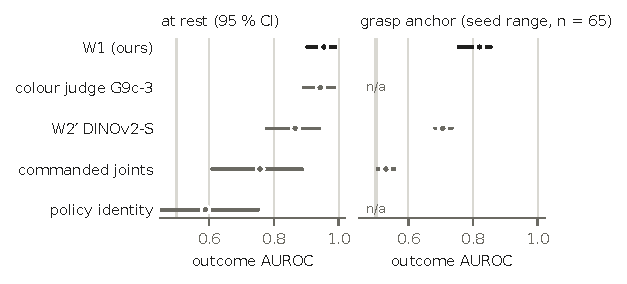
\includegraphics[width=\columnwidth]{fig/table2.pdf}
\caption{The controls table as a dot plot. Left: AUROC at rest with its 95 \% bootstrap CI. Right: AUROC at the grasp anchor, mean of 5 seeds with the seed range (not a CI). Exploratory, LOSO, operator labels.}\label{fig:controls}
\end{figure}
In this exploratory comparison on the 69 rollouts, our world model is level with the colour judge at rest (the CIs overlap) and above the frozen encoder and the joints; at the grasp anchor, where no judge applies, it leads both controls. The anchor column depends on how the seeds are aggregated (exploratory): the AUROC of the 5-seed-averaged predictions is 0.8377 / 0.7175 / 0.5346 (ours / frozen DINOv2-S / joints), and seed 0 alone gives 0.7554 / 0.7024 / 0.5574, a smaller gap between our model and the frozen encoder; the ordering holds in both. The pose probes hold the joints better than our encoder does but the outcome worse, so on these rollouts the encoder holds outcome information they do not (exploratory). The original outcome-readout gate scored our model at 1.000, but against the colour judge's labels rather than the operator's, on 87 rollouts; the rerun here, on the 69 Orin rollouts against operator labels with the controls beside it, gives 0.9545.
\section{Where the predictor fails}
The cleanest contrast is the grasp probe, which ContactGuard~\citep{zheng2026contactguard} motivates: same encoder, same anchor, current latent 0.82 against imagined latent 0.70, where the bar was $\geq$ 0.85, $\geq$ +0.05 over the current latent. On these rollouts, imagining forward loses outcome information the encoder had; this pre-registered row fails, and the encoder/predictor reading built on it stays exploratory. On SURVEYOR's scale check, the frozen DINOv2-S control ($\tau$ 0.3601) and the joints ($\tau$ 0.0265) pass where our model fails, which points at our model's latent geometry rather than the task.
\emph{Three further exploratory lines.} (1) On the inverse-dynamics term of the distillation probe (pooled, 25 teleoperation validation episodes), the trained model (0.7476) is not distinguishable from its own random initialisation (0.7974): the difference is −0.0499, with a 95 \% paired episode-bootstrap CI of [−0.7403, +0.6559] (\texttt{gap5\_pooled\_rerun.json}). The term is sensitive to BLAS and ridge conditioning: the same untrained network scored 1.4383 on one machine and 0.7974 / 0.8042 on two others. (2) The surprise scorer that gives our model a failure-class AUROC of 0.775, below its sanity bar, reproduces the open-loop corruption ratios at K = 30 (cross-episode 3.428 vs 3.341, constant-first 2.558 vs 2.543; \texttt{M1\_diag\_g0\_repro.json}), so that AUROC is a real value and not a load or scorer bug. (3) The predictor of VLA-JEPA is close to action-blind (exploratory, 5 anchors; Table~\ref{tab:vlajepa}): action tokens from another episode change the tokens by 21--28 \% (relative L2) and the loss by about 0.05 \%; zeroing the tokens changes the loss by about 1.05 \% on average (|Δ| 0.4--2.2 \%), and the forward pass is deterministic. Its failure-class AUROC of 0.501, below the same sanity bar, is therefore a real value, and its table stays unread under the frozen bar.
\begin{table}[!t]\centering\setlength{\tabcolsep}{3pt}\scriptsize
\caption{VLA-JEPA world-model loss at 5 anchors with the true action tokens, tokens from another episode (Δ shuffled) and zeroed tokens; the token change is the relative L2 of the shuffled tokens. Exploratory, a spot check, not a power analysis. Source: repro/gaps/expected/M3\_diag\_action\_shuffle.json.}\label{tab:vlajepa}
\resizebox{\columnwidth}{!}{\begin{tabular}{lllll}
\toprule
\shissohead anchor (episode / frame) & true loss & Δ shuffled (\%) & token change (\%) & Δ zeroed (\%) \\
\midrule
8 / 402 & 1.3031 & +0.014 & 21.1 & +2.22 \\
10 / 227 & 1.4641 & +0.088 & 27.6 & +0.50 \\
23 / 327 & 1.4215 & +0.036 & 21.1 & +0.87 \\
59 / 302 & 1.4637 & +0.030 & 25.5 & +1.28 \\
65 / 302 & 1.5236 & −0.070 & 22.0 & −0.38 \\
\bottomrule
\end{tabular}}
\end{table}
\emph{Objection: the anticipation step of the outcome-readout gate is a predictive pass.} There the imagined latent beat policy identity by +0.179, but that bar is retrospective, and the two bar-first reruns of the same idea, the grasp probe and the calibrated surprise reflex, both fail.
\section{Related work}
LeWorldModel~\citep{maes2026lewm} trains the JEPA recipe we use end to end from pixels and plans with it in Push-T and in simulation; its planning uses fail here (chunk ranking, re-ranking). The identifiability analysis of LeJEPA~\citep{klindt2026lejepa} predicts that SIGReg latents identify the state up to anisotropy, which holds here partially. DINO-WM~\citep{zhou2024dinowm} plans on frozen DINOv2~\citep{oquab2023dinov2} patches, the design of our frozen control. V-JEPA 2.1~\citep{murlabadia2026vjepa21} and RoboJEPA~\citep{zholus2026robojepa} are too slow on our on-board computer. ContactGuard~\citep{zheng2026contactguard} finds that imagined-latent probes beat current-latent ones on grasp tasks; we find the opposite. ReAP~\citep{liu2026reap} predicts action-conditioned risk, and its re-test misses its bar here, as do the hierarchical planners of HWM~\citep{zhang2026hwm} and H-JEPA~\citep{zhang2026hjepa} and the latent-distance scale of SURVEYOR~\citep{surveyor2026}. Two results agree with ours from the control side: SaiVLA-JEPA~\citep{xiao2026saivla} finds that a training-only future-latent head adds +0.03 points to control on 10,030 paired episodes, and HIJP~\citep{hijp2026} finds LeWM below goal-conditioned behaviour cloning in simulation.
\section{Limitations}
The controls are exploratory: 69 rollouts, operator labels, probes chosen after the data. Fresh rollouts scored under a bar committed first are the test, and until it runs every statement of the encoder/predictor split above is exploratory. One rig, one model, one data scale: a second scale point (653 episodes) is costed and queued separately, and the scale curve belongs to a longer version. Not run: the surprise monitor and the imagined-latent grasp probe with the frozen DINOv2-S control or the joints (each needs its own predictor), and progress monotonicity with the controls (it needs a reimplementation). The bar of the outcome-readout use is retrospective, and the one same-commit bar is that of the two-level hierarchical progress use.
\section{Conclusion}
On a small teleoperation dataset, a JEPA world model learns an encoder that reads how the episode went, a short horizon ahead included, and, in exploratory probes on the 69 rollouts, a predictor whose imagination adds nothing to that reading. Reporting every pre-registered use, not the best one, is what makes that visible.
\bibliographystyle{unsrtnat}
\bibliography{refs}
\end{document}
